\chapter{Diagrammes de Feynman}\label{annexe-fmf}
\begin{wrapfigure}{R}{5.75cm}
\centering
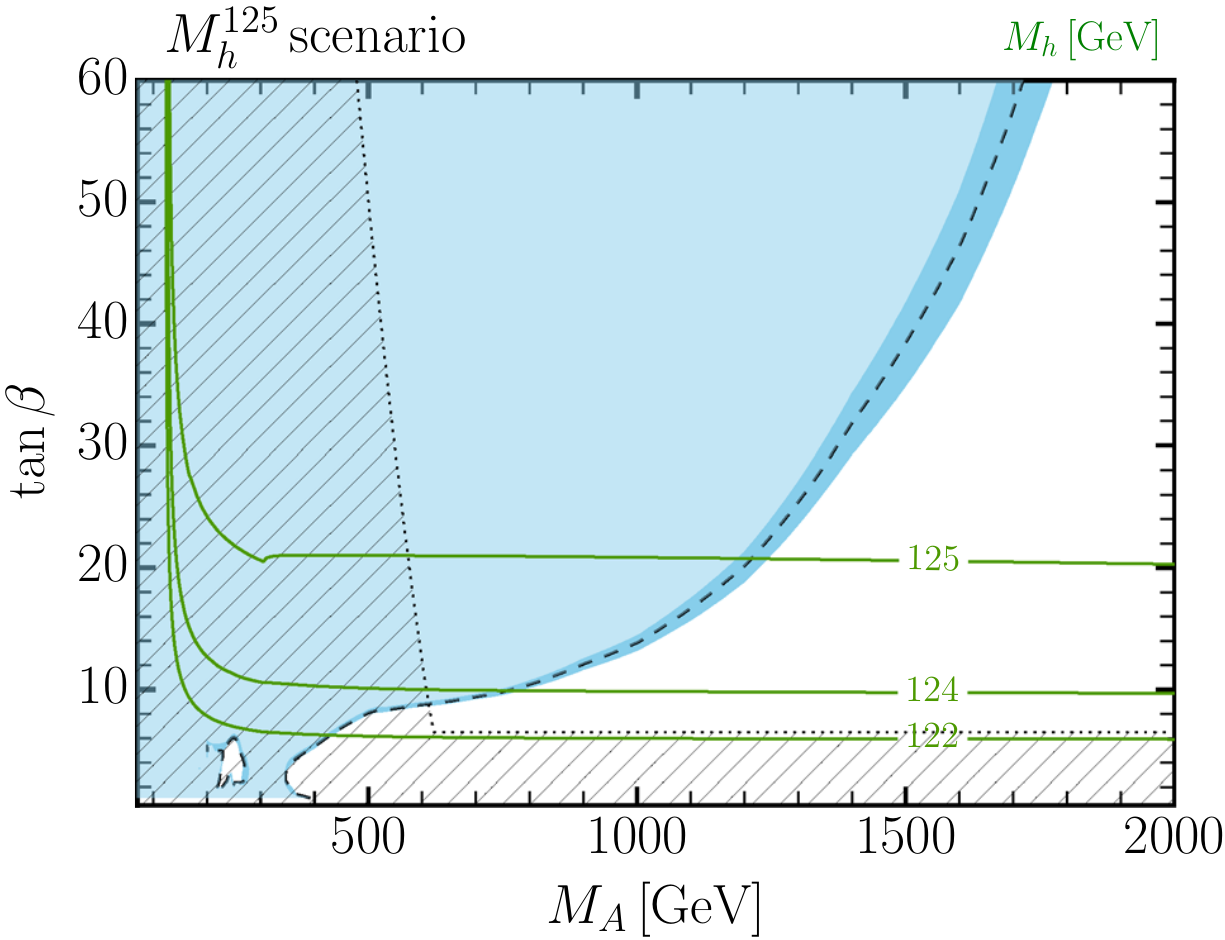
\includegraphics[width=\linewidth]{\PhDthesisdir/plots_and_images/from_Feynman_diagrams_1/fig1.png}
\caption[Diagramme de Feynman de la diffusion électron-électron.]{Diagramme de Feynman de la diffusion électron-électron présenté dans la référence~\cite{Feynman_diagrams_1}. Ici, le temps s'écoule vers le haut; l'état initial est donc en bas du diagramme et l'état final en haut.}
\label{fig-first_Feynman_diag-annexeB}
\end{wrapfigure}
Les diagrammes de Feynman sont des représentations graphiques des équations mathématiques, issues de la théorie quantique des champs, décrivant les interactions entre particules.
Grâce à leur aspect visuel simple, ils permettent une approche intuitive de ces équations souvent complexes.
Ces diagrammes ont été inventés par Richard Feynman à la fin des années 40 afin de réaliser des calculs de diffusion de particules~\cite{Feynman_diagrams_1}.
Un des tout premiers diagrammes de Feynman présents dans la littérature représente ainsi la diffusion entre deux électrons.
Il se trouve sur la figure~\ref{fig-first_Feynman_diag-annexeB}.
Le temps s'y écoule de bas en haut; l'état initial est donc en bas du diagramme et l'état final en haut.
Dans les diagrammes de Feynman du reste de cette thèse, le temps s'écoule de gauche à droite.
Ainsi, l'état initial se trouve à gauche et l'état final à droite.
\par Les diagrammes de Feynman ne représentent pas pour autant la réalité physique des processus étudiés.
En effet, seuls les états initiaux et finaux sont réels, les parties internes de chaque diagramme correspondant aux manières de passer d'un état à l'autre.
Il faut prendre en compte plusieurs diagrammes de Feynman, parfois de plus en plus complexes, \ie\ d'ordres supérieurs, afin d'obtenir une description fidèle du processus étudié.
\par Ainsi, pour un processus de type $\positron\electron\to\positron\electron$, \ie\
un état initial contenant
un anti-électron d'impulsion $\vec{p}_1$
et
un électron d'impulsion $\vec{p}_2$
et
un état final contenant
un anti-électron d'impulsion $\vec{p}_3$
et
un électron d'impulsion $\vec{p}_4$,
l'étude complète du phénomène physique (membre de gauche sur la figure~\ref{fig-several_fmfs-annexeB}) doit prendre en compte la diffusion (premier terme du membre de droite), l'annihilation et réapparition de la paire $\positron\electron$ par interaction électromagnétique (second terme) ou faible (troisième terme) et aussi des processus plus complexes (quatrième et cinquième termes).
\begin{figure}[h]
\centering
\vspace{\baselineskip}
\begin{tikzpicture}
\draw (0,0) node (equal) {\Large =};
\draw (equal.west) node [left] {\ \ \begin{fmffile}{ee_to_ee_global}\fmfstraight
\begin{fmfchar*}(20,20)
  \fmfleft{i1,i2}
  \fmfright{o1,o2}
  \fmf{fermion}{i1,v1,i2}
  \fmf{fermion}{o2,v1,o1}
  \fmflabel{\antiele}{i2}
  \fmflabel{\electron}{i1}
  \fmflabel{\antiele}{o2}
  \fmflabel{\electron}{o1}
  \fmfblob{.5w}{v1}
\end{fmfchar*}
\end{fmffile}\ \ };

\draw (equal.east) node (d1) [right] {\ \ \begin{fmffile}{ee_gamma_ee_t}\fmfstraight
\begin{fmfchar*}(20,20)
  \fmfleft{i1,i2}
  \fmfright{o1,o2}
  \fmf{fermion}{i1,v1,o1}
  \fmf{fermion}{o2,v2,i2}
  \fmf{photon, label=\photon, l.side=left}{v1,v2}
  \fmflabel{\antiele}{i2}
  \fmflabel{\electron}{i1}
  \fmflabel{\antiele}{o2}
  \fmflabel{\electron}{o1}
  \fmfdot{v1,v2}
\end{fmfchar*}
\end{fmffile}\ \ };
\draw (d1.east) node (p) [right] {\Large +};
\draw (p.east) node (d) [right] {\ \ \begin{fmffile}{ee_gamma_ee_s}\fmfstraight
\begin{fmfchar*}(20,20)
  \fmfleft{i1,i2}
  \fmfright{o1,o2}
  \fmf{fermion}{i1,v1,i2}
  \fmf{fermion}{o2,v2,o1}
  \fmf{photon, label=\photon, l.side=left}{v1,v2}
  \fmflabel{\antiele}{i2}
  \fmflabel{\electron}{i1}
  \fmflabel{\antiele}{o2}
  \fmflabel{\electron}{o1}
  \fmfdot{v1,v2}
\end{fmfchar*}
\end{fmffile}\ \ };
\draw (d.east) node (p) [right] {\Large +};
\draw (p.east) node (d) [right] {\ \ \begin{fmffile}{ee_Z_ee_s}\fmfstraight
\begin{fmfchar*}(20,20)
  \fmfleft{i1,i2}
  \fmfright{o1,o2}
  \fmf{fermion}{i1,v1,i2}
  \fmf{fermion}{o2,v2,o1}
  \fmf{boson, label=\Zboson, l.side=left}{v1,v2}
  \fmflabel{\antiele}{i2}
  \fmflabel{\electron}{i1}
  \fmflabel{\antiele}{o2}
  \fmflabel{\electron}{o1}
  \fmfdot{v1,v2}
\end{fmfchar*}
\end{fmffile}\ \ };
%\draw (d.east) node (p) [right] {\Large +};
%\draw (p.east) node (d) [right] {\ldots};

\draw (equal.south east)+(0,-6\baselineskip) node (p) {\Large +};
\draw (p.east) node (d) [right] {\ \ \begin{fmffile}{ee_WW_ee_1}\fmfstraight
\begin{fmfchar*}(30,10)
  \fmfleft{i1,i2}
  \fmfright{o1,o2}
  \fmf{fermion}{i1,v1}
  \fmf{boson, label=\Wbosonminus, l.side=right}{v1,v4}
  \fmf{fermion}{v4,o1}
  \fmf{fermion}{o2,v3}
  \fmf{boson, label=\Wbosonplus, l.side=left}{v2,v3}
  \fmf{fermion}{v2,i2}
  \fmffreeze
  \fmf{fermion, label=\nuele, l.side=left}{v1,v2}
  \fmf{fermion, label=\nuele, l.side=left}{v3,v4}
  \fmflabel{\antiele}{i2}
  \fmflabel{\electron}{i1}
  \fmflabel{\antiele}{o2}
  \fmflabel{\electron}{o1}
  \fmfdot{v1,v2,v3,v4}
\end{fmfchar*}
\end{fmffile}\ \ };
\draw (d.east) node (p) [right] {\Large +};
\draw (p.east) node (d) [right] {\ \ \begin{fmffile}{ee_WW_ee_2}\fmfstraight
\begin{fmfchar*}(30,10)
  \fmfleft{i1,i2}
  \fmfright{o1,o2}
  \fmf{fermion}{i1,v1}
  \fmf{fermion, label=\nuele, l.side=right}{v1,v4}
  \fmf{fermion}{v4,o1}
  \fmf{fermion}{o2,v3}
  \fmf{fermion, label=\antinuele, l.side=right}{v3,v2}
  \fmf{fermion}{v2,i2}
  \fmffreeze
  \fmf{boson, label=\Wboson, l.side=left}{v1,v2}
  \fmf{boson, label=\Wboson, l.side=left}{v3,v4}
  \fmflabel{\antiele}{i2}
  \fmflabel{\electron}{i1}
  \fmflabel{\antiele}{o2}
  \fmflabel{\electron}{o1}
  \fmfdot{v1,v2,v3,v4}
\end{fmfchar*}
\end{fmffile}\ \ };
\draw (d.east) node (p) [right] {\Large +};
\draw (p.east) node (d) [right] {\ldots};
\end{tikzpicture}
\vspace{\baselineskip}
\caption[Prise en compte de plusieurs diagrammes de Feynman.]{Prise en compte de plusieurs diagrammes de Feynman lors de l'étude d'un processus physique donné.}
\label{fig-several_fmfs-annexeB}
\end{figure}
\pagebreak
\par Selon le type de particule se propageant (fermion, photon, boson de Higgs ...), différents types de lignes sont utilisés dans les diagrammes de Feynman.
Plusieurs conventions existent, en particulier pour les bosons.
La convention utilisée dans cette thèse est illustrée sur la figure~\ref{fig-fmf_lines_convention-annexeB}.
\begin{figure}[h]
\centering
\begin{tikzpicture}
\draw (0,0) coordinate (current);

\foreach \file/\name/\sname in {fermion/fermion/,antifermion/antifermion/,gluon/gluon/,boson_vecteur/boson vecteur/{(\photon, \Wbosonpm, \Zboson)},boson_scalaire/boson scalaire/(Higgs)} {

\draw (current.east) node [right] (diagram) {\qquad \ \input{\PhDthesisdir/plots_and_images/Feynman_diagrams/drawing_conventions/fgraph-\file.tex}\qquad \ };

\draw (diagram.south) node (name) [below] {\name};
\draw (name.south) node [below] {\sname};

\draw (diagram.east) coordinate (current);
}
\end{tikzpicture}
\caption[Types de particules et lignes correspondantes dans les diagrammes de Feynman.]{Types de particules et lignes correspondantes dans les diagrammes de Feynman.}
\label{fig-fmf_lines_convention-annexeB}
\end{figure}
\par Les interactions entre les particules ont lieu, dans les diagrammes de Feynman, au niveau des connexions entre les lignes correspondant à ces particules.
Ces connexions sont les \og vertex \fg{} du diagramme.
Dans le cadre de la théorie quantique des champs, les interactions entre les particules sont possibles grâce aux termes du lagrangien faisant intervenir les champs correspondants à ces particules.
Par exemple, dans le cas de l'interaction électromagnétique abordée dans le chapitre~\ifref{chapter-MS-MSSM}{\ref{chapter-MS-MSSM}}{2}, un des termes du lagrangien est
\begin{equation}
\bar{\psi}\gamma^\mu eQA_\mu \psi
=
\bar{\psi}_a \,\, [\gamma^\mu]_{ab} \, eQ \,\, A_\mu \,\, \psi_b
\mend[,]
\label{eq-QCD_interaction_developped}
\end{equation}
faisant intervenir le champ $\psi$ des fermions, $\bar{\psi}$ pour les antifermions ainsi que le champ $A_\mu$ des photons.
Ce terme du lagrangien correspond directement aux vertex comme celui de la figure~\ref{fig-fgraph-ff_Gamma1-large-annexeB}, sur laquelle les rôles des différents facteurs présents dans ce terme du lagrangien sont illustrés.
\begin{figure}[h]
\centering
\vspace{\baselineskip}
\begin{fmffile}{ff_Gamma1-large_with_annotations}\fmfstraight
\begin{fmfchar*}(40,40)
  \fmfleft{i1,i2}
  \fmfright{o1}
  \fmf{fermion, label=$\psi_b$, l.side=right}{i1,v}
  \fmf{fermion, label=$\bar{\psi}_a$}{v,i2}
  \fmf{photon, label=$A_\mu$}{v,o1}
  \fmflabel{\fermion}{i1}
  \fmflabel{\antifermion}{i2}
  \fmflabel{\photon}{o1}
  \fmflabel{$eQ\gamma^\mu_{ab}\longrightarrow$}{v}
  \fmfdot{v}
\end{fmfchar*}
\end{fmffile}
\vspace{\baselineskip}
\caption[Diagramme de Feynman issu du terme~\eqref{eq-QCD_interaction_developped}.]{Diagramme de Feynman issu du terme du lagrangien du modèle standard de l'équation~\eqref{eq-QCD_interaction_developped}. Un fermion \fermion\ et un antifermion \antifermion\ sont présents dans l'état initial et sont décrits par un champ fermionique $\psi$ et son adjoint $\bar{\psi}$. Le champ $\psi$ interagit par ses composantes $a$ et $b$ avec le champ vectoriel $A_\mu$ au vertex, avec un couplage donné par $eQ\gamma^\mu_{ab}$. Il en résulte un photon \photon, décrit par ce champ $A_\mu$.}
\label{fig-fgraph-ff_Gamma1-large-annexeB}
\end{figure}
\par Les diagrammes de Feynman ainsi obtenus sont un outil incontournable en physique des particules.
En physique nucléaire et en physique de la matière condensée, le formalisme étant proche de celui de la physique des particules, des analogues des diagrammes de Feynman sont également utilisés.